\documentclass{article}
\title{Современные методы анализа и применения современных методов анализов и применений в контексте применения современных методов упрощения и приведения к упрощенному виду выражений, примененных к анализу современных методов}
\date{2077-95-07}
\author{Albert Einstein}
\usepackage[T2A]{fontenc}
\usepackage[utf8]{inputenc}
\usepackage[russian]{babel}
\usepackage{amsmath}
\usepackage{graphicx}
\usepackage{hyperref}
\usepackage{xcolor}
\usepackage[legalpaper,portrait,margin=1in]{geometry}
\begin{document}
\maketitle
\newpage
\allowdisplaybreaks
\section{Введение}В современной мифологии большое значение имеют пробки на дорогах в Азербайджане. Лучшие аналитики и профессиональные тавтологи изучили эту проблему и результатом их работы стала формула, совершившая прорыв в науке, а в особенности - в области Нижневартовска. В этой статье приведен способ упрощения и приведения к каноническому виду данной формулы.\section{Упрощение}\begin{center}Изначально имеем формулу\begin{gather*}
{{\frac{{d}}{{d{{x}}}}}{{\left({{x}^{\sin{{x}}}}+{{{{\ln{{7}}}{{x}^{\sin{{x}}}}}{\left(-{1}\right)}}{\left({\frac{{x}}{{x}}}+{1}\right)}}\right)}}}\end{gather*}
Я все делал по науке, и у меня не получилось... Ну да плевать\begin{gather*}
{{\frac{{d}}{{d{{x}}}}}{{\left({{x}^{\sin{{x}}}}+{{\ln{{7}}}{{{x}^{\sin{{x}}}}{\cdot}{{\left({\color{red}{{\frac{{{1}{{x}^{\left({1}-{{1}{\cdot}{1}}\right)}}}}{{{1}{{x}^{\left({1}-{{1}{\cdot}{1}}\right)}}}}}}}+{1}\right)}{\left(-{1}\right)}}}}\right)}}}\end{gather*}
Интеграл пока написал без пределов, но этот беспредел мы скоро устраним.\begin{gather*}
{{\frac{{d}}{{d{{x}}}}}{{\left({{x}^{\sin{{x}}}}+{{\ln{{7}}}{{{x}^{\sin{{x}}}}{\color{red}{{\left({{\left(-{1}\right)}{\cdot}{\left(\frac{{{1}{{x}^{\left({1}-{1}\right)}}}}{{{1}{{x}^{\left({1}-{{1}{\cdot}{1}}\right)}}}}\right)}}+{{\left(-{1}\right)}{\cdot}{1}}\right)}}}}}\right)}}}\end{gather*}
Это не единица, это ноль, здесь единиц не бывает\begin{gather*}
{{\frac{{d}}{{d{{x}}}}}{{\left({{x}^{\sin{{x}}}}+{{\ln{{7}}}{{{x}^{\sin{{x}}}}{\left({{\left(-{1}\right)}{\cdot}{\left(\frac{{{1}{{x}^{\color{red}{{\left({-{1}}+{1}\right)}}}}}}{{{1}{{x}^{\left({1}-{{1}{\cdot}{1}}\right)}}}}\right)}}+{{\left(-{1}\right)}{\cdot}{1}}\right)}}}\right)}}}\end{gather*}
Сделаем вид, что вам понятно\begin{gather*}
{{\frac{{d}}{{d{{x}}}}}{{\left({{x}^{\sin{{x}}}}+{{\ln{{7}}}{{{x}^{\sin{{x}}}}{\left({{\left(-{1}\right)}{\cdot}{\left(\frac{{{1}{{x}^{\color{red}{{\left(-{0}\right)}}}}}}{{{1}{{x}^{\left({1}-{{1}{\cdot}{1}}\right)}}}}\right)}}+{{\left(-{1}\right)}{\cdot}{1}}\right)}}}\right)}}}\end{gather*}
Наука всегда победит\begin{gather*}
{{\frac{{d}}{{d{{x}}}}}{{\left({{x}^{\sin{{x}}}}+{{\ln{{7}}}{{{x}^{\sin{{x}}}}{\left({{\left(-{1}\right)}{\cdot}{\left(\frac{{\color{red}{{1}}}}{{{1}{{x}^{\left({1}-{{1}{\cdot}{1}}\right)}}}}\right)}}+{{\left(-{1}\right)}{\cdot}{1}}\right)}}}\right)}}}\end{gather*}
Первая производная позволяет определить скорость возрастание/убывания функции. Вторая производная определяет выпуклость, а третья - скорость взятия студентом производных.\begin{gather*}
{{\frac{{d}}{{d{{x}}}}}{{\left({{x}^{\sin{{x}}}}+{{\ln{{7}}}{{{x}^{\sin{{x}}}}{\left({{\left(-{1}\right)}{\cdot}{\left(\frac{{1}}{{{1}{{x}^{\color{red}{{\left({1}-{1}\right)}}}}}}\right)}}+{{\left(-{1}\right)}{\cdot}{1}}\right)}}}\right)}}}\end{gather*}
Всё, больше не буду ничего делать\begin{gather*}
{{\frac{{d}}{{d{{x}}}}}{{\left({{x}^{\sin{{x}}}}+{{\ln{{7}}}{{{x}^{\sin{{x}}}}{\left({{\left(-{1}\right)}{\cdot}{\left(\frac{{1}}{{{1}{{x}^{\color{red}{{\left({-{1}}+{1}\right)}}}}}}\right)}}+{{\left(-{1}\right)}{\cdot}{1}}\right)}}}\right)}}}\end{gather*}
Это бан.\begin{gather*}
{{\frac{{d}}{{d{{x}}}}}{{\left({{x}^{\sin{{x}}}}+{{\ln{{7}}}{{{x}^{\sin{{x}}}}{\left({{\left(-{1}\right)}{\cdot}{\left(\frac{{1}}{{{1}{{x}^{\color{red}{{\left(-{0}\right)}}}}}}\right)}}+{{\left(-{1}\right)}{\cdot}{1}}\right)}}}\right)}}}\end{gather*}
Отправим производную в коллайдер\begin{gather*}
{{\frac{{d}}{{d{{x}}}}}{{\left({{x}^{\sin{{x}}}}+{{\ln{{7}}}{{{x}^{\sin{{x}}}}{\left({\color{red}{{-{1}}}}+{{\left(-{1}\right)}{\cdot}{1}}\right)}}}\right)}}}\end{gather*}
Я записал такую формулу. Это мой выбор\begin{gather*}
{{\frac{{d}}{{d{{x}}}}}{{\left({{x}^{\sin{{x}}}}+{{\ln{{7}}}{{{x}^{\sin{{x}}}}{\left({-{1}}-{1}\right)}}}\right)}}}\end{gather*}
Квадрат - это не треугольник на стероидах, это отдельная фигура\begin{gather*}
{{\frac{{d}}{{d{{x}}}}}{{\left({{x}^{\sin{{x}}}}+{{\ln{{7}}}{{{x}^{\sin{{x}}}}{\color{red}{{\left(-{2}\right)}}}}}\right)}}}\end{gather*}
Формула красивая, но бесполезная\begin{gather*}
{{\frac{{d}}{{d{{x}}}}}{{\color{red}{{{{x}^{\left({\sin{{x}}}{\cdot}{1}\right)}}{\cdot}{\left({{{1}^{\sin{{x}}}}{{x}^{\left({\sin{{x}}}-{{\sin{{x}}}{\cdot}{1}}\right)}}}+{{\ln{{7}}}{\cdot}{{{{1}^{\sin{{x}}}}{{x}^{\left({\sin{{x}}}-{{\sin{{x}}}{\cdot}{1}}\right)}}}{\left(-{2}\right)}}}\right)}}}}}}\end{gather*}
Бесконечно малую величину запрем в ванной\begin{gather*}
{{\frac{{d}}{{d{{x}}}}}{{{{x}^{\color{red}{{\sin{{x}}}}}}{\cdot}{\left({{{1}^{\sin{{x}}}}{{x}^{\left({\sin{{x}}}-{{\sin{{x}}}{\cdot}{1}}\right)}}}+{{\ln{{7}}}{\cdot}{{{{1}^{\sin{{x}}}}{{x}^{\left({\sin{{x}}}-{{\sin{{x}}}{\cdot}{1}}\right)}}}{\left(-{2}\right)}}}\right)}}}}\end{gather*}
После взрыва останется\begin{gather*}
{{\frac{{d}}{{d{{x}}}}}{{{{x}^{\sin{{x}}}}{\cdot}{\left({{\color{red}{{1}}}{{x}^{\left({\sin{{x}}}-{{\sin{{x}}}{\cdot}{1}}\right)}}}+{{\ln{{7}}}{\cdot}{{{{1}^{\sin{{x}}}}{{x}^{\left({\sin{{x}}}-{{\sin{{x}}}{\cdot}{1}}\right)}}}{\left(-{2}\right)}}}\right)}}}}\end{gather*}
Просто взять эту симплициальную резольвенту, взять её абеленизацию, и вот окажется, что гомотопические группы абленизации резольвенты это как раз таки целочисленные гомологии нашей группы G.\begin{gather*}
{{\frac{{d}}{{d{{x}}}}}{{{{x}^{\sin{{x}}}}{\cdot}{\left({{1}{{x}^{\color{red}{{\left({\sin{{x}}}-{\sin{{x}}}\right)}}}}}+{{\ln{{7}}}{\cdot}{{{{1}^{\sin{{x}}}}{{x}^{\left({\sin{{x}}}-{{\sin{{x}}}{\cdot}{1}}\right)}}}{\left(-{2}\right)}}}\right)}}}}\end{gather*}
Я больше решать не буду, уже сколько можно\begin{gather*}
{{\frac{{d}}{{d{{x}}}}}{{{{x}^{\sin{{x}}}}{\cdot}{\left({{1}{{x}^{\left({\sin{{x}}}+{\color{red}{{{\left(-{1}\right)}{\sin{{x}}}}}}\right)}}}+{{\ln{{7}}}{\cdot}{{{{1}^{\sin{{x}}}}{{x}^{\left({\sin{{x}}}-{{\sin{{x}}}{\cdot}{1}}\right)}}}{\left(-{2}\right)}}}\right)}}}}\end{gather*}
Формула красивая, но бесполезная\begin{gather*}
{{\frac{{d}}{{d{{x}}}}}{{{{x}^{\sin{{x}}}}{\cdot}{\left({{1}{{x}^{\left({\sin{{x}}}+{\color{red}{{{\sin{{x}}}{\left(-{1}\right)}}}}\right)}}}+{{\ln{{7}}}{\cdot}{{{{1}^{\sin{{x}}}}{{x}^{\left({\sin{{x}}}-{{\sin{{x}}}{\cdot}{1}}\right)}}}{\left(-{2}\right)}}}\right)}}}}\end{gather*}
Кто придумывал эту задачу?...\begin{gather*}
{{\frac{{d}}{{d{{x}}}}}{{{{x}^{\sin{{x}}}}{\cdot}{\left({{1}{{x}^{\color{red}{{\left({\sin{{x}}}{\left({-{1}}+{1}\right)}\right)}}}}}+{{\ln{{7}}}{\cdot}{{{{1}^{\sin{{x}}}}{{x}^{\left({\sin{{x}}}-{{\sin{{x}}}{\cdot}{1}}\right)}}}{\left(-{2}\right)}}}\right)}}}}\end{gather*}
Кто придумывал эту задачу?...\begin{gather*}
{{\frac{{d}}{{d{{x}}}}}{{{{x}^{\sin{{x}}}}{\cdot}{\left({{1}{{x}^{\left({\sin{{x}}}{\color{red}{{\left(-{0}\right)}}}\right)}}}+{{\ln{{7}}}{\cdot}{{{{1}^{\sin{{x}}}}{{x}^{\left({\sin{{x}}}-{{\sin{{x}}}{\cdot}{1}}\right)}}}{\left(-{2}\right)}}}\right)}}}}\end{gather*}
Применим простую замену\begin{gather*}
{{\frac{{d}}{{d{{x}}}}}{{{{x}^{\sin{{x}}}}{\cdot}{\left({\color{red}{{1}}}+{{\ln{{7}}}{\cdot}{{{{1}^{\sin{{x}}}}{{x}^{\left({\sin{{x}}}-{{\sin{{x}}}{\cdot}{1}}\right)}}}{\left(-{2}\right)}}}\right)}}}}\end{gather*}
Это безобразие причешем вдальнейшем до\begin{gather*}
{{\frac{{d}}{{d{{x}}}}}{{{{x}^{\sin{{x}}}}{\cdot}{\left({1}+{{\ln{{7}}}{\cdot}{{\color{red}{{1}}}{{{x}^{\left({\sin{{x}}}-{{\sin{{x}}}{\cdot}{1}}\right)}}{\left(-{2}\right)}}}}\right)}}}}\end{gather*}
Итак\begin{gather*}
{{\frac{{d}}{{d{{x}}}}}{{{{x}^{\sin{{x}}}}{\cdot}{\left({1}+{{\ln{{7}}}{\cdot}{{1}{{{x}^{\color{red}{{\left({\sin{{x}}}-{\sin{{x}}}\right)}}}}{\left(-{2}\right)}}}}\right)}}}}\end{gather*}
Итак\begin{gather*}
{{\frac{{d}}{{d{{x}}}}}{{{{x}^{\sin{{x}}}}{\cdot}{\left({1}+{{\ln{{7}}}{\cdot}{{1}{{{x}^{\left({\sin{{x}}}+{\color{red}{{{\left(-{1}\right)}{\sin{{x}}}}}}\right)}}{\left(-{2}\right)}}}}\right)}}}}\end{gather*}
Зря я вообще это написал, это не объясняет, а ухудшает\begin{gather*}
{{\frac{{d}}{{d{{x}}}}}{{{{x}^{\sin{{x}}}}{\cdot}{\left({1}+{{\ln{{7}}}{\cdot}{{1}{{{x}^{\left({\sin{{x}}}+{\color{red}{{{\sin{{x}}}{\left(-{1}\right)}}}}\right)}}{\left(-{2}\right)}}}}\right)}}}}\end{gather*}
Я не хочу брать произведение, ну его в болото\begin{gather*}
{{\frac{{d}}{{d{{x}}}}}{{{{x}^{\sin{{x}}}}{\cdot}{\left({1}+{{\ln{{7}}}{\cdot}{{1}{{{x}^{\color{red}{{\left({\sin{{x}}}{\left({-{1}}+{1}\right)}\right)}}}}{\left(-{2}\right)}}}}\right)}}}}\end{gather*}
Здесь могла быть ваша реклама\begin{gather*}
{{\frac{{d}}{{d{{x}}}}}{{{{x}^{\sin{{x}}}}{\cdot}{\left({1}+{{\ln{{7}}}{\cdot}{{1}{{{x}^{\left({\sin{{x}}}{\color{red}{{\left(-{0}\right)}}}\right)}}{\left(-{2}\right)}}}}\right)}}}}\end{gather*}
Здесь могла быть ваша реклама\begin{gather*}
{{\frac{{d}}{{d{{x}}}}}{{{{x}^{\sin{{x}}}}{\cdot}{\left({1}+{{\ln{{7}}}{\cdot}{{1}{\cdot}{{\color{red}{{1}}}{\left(-{2}\right)}}}}\right)}}}}\end{gather*}
Это бан.\begin{gather*}
{{\frac{{d}}{{d{{x}}}}}{{{{x}^{\sin{{x}}}}{\cdot}{\left({1}+{\color{red}{{{\ln{{7}}}{{\left(-{2}\right)}{\cdot}{{1}{\cdot}{1}}}}}}\right)}}}}\end{gather*}
Сотру, чтобы нарисовать примерно то же самое\begin{gather*}
{{\frac{{d}}{{d{{x}}}}}{{{{x}^{\sin{{x}}}}{\cdot}{\left({1}+{{\ln{{7}}}{\color{red}{{\left(-{2}\right)}}}}\right)}}}}\end{gather*}
Сократим числитель и степень и получим\begin{gather*}
{{\frac{{d}}{{d{{x}}}}}{{{{x}^{\sin{{x}}}}{\color{red}{{\left({{\ln{{7}}}{\left(-{2}\right)}}+{1}\right)}}}}}}\end{gather*}
Раскроем знак производной и получим\begin{gather*}
{\color{red}{{{{{x}^{\sin{{x}}}}{\left({\frac{{d}}{{d{{x}}}}}{{\left({{\ln{{7}}}{\left(-{2}\right)}}+{1}\right)}}\right)}}+{{\left({\frac{{d}}{{d{{x}}}}}{{{x}^{\sin{{x}}}}}\right)}{\left({{\ln{{7}}}{\left(-{2}\right)}}+{1}\right)}}}}}\end{gather*}
Возьмем производную и получим\begin{gather*}
{{{{x}^{\sin{{x}}}}{\color{red}{{\left({{\frac{{d}}{{d{{x}}}}}{{{\ln{{7}}}{\left(-{2}\right)}}}}+{{\frac{{d}}{{d{{x}}}}}{{1}}}\right)}}}}+{{\left({\frac{{d}}{{d{{x}}}}}{{{x}^{\sin{{x}}}}}\right)}{\left({{\ln{{7}}}{\left(-{2}\right)}}+{1}\right)}}}\end{gather*}
Раскроем дифференциал и получим\begin{gather*}
{{{{x}^{\sin{{x}}}}{\left({{\ln{{7}}}{\left({\frac{{d}}{{d{{x}}}}}{{\left(-{2}\right)}}\right)}}+{\color{red}{{{{\left({\frac{{d}}{{d{{x}}}}}{{\ln{{7}}}}\right)}{\left(-{2}\right)}}+{{\frac{{d}}{{d{{x}}}}}{{1}}}}}}\right)}}+{{\left({\frac{{d}}{{d{{x}}}}}{{{x}^{\sin{{x}}}}}\right)}{\left({{\ln{{7}}}{\left(-{2}\right)}}+{1}\right)}}}\end{gather*}
Самое время раскрыть производную и получить\begin{gather*}
{{{{x}^{\sin{{x}}}}{\left({{\ln{{7}}}{\color{red}{{\left(-{\left({\frac{{d}}{{d{{x}}}}}{{2}}\right)}\right)}}}}+{{{\left({\frac{{d}}{{d{{x}}}}}{{\ln{{7}}}}\right)}{\left(-{2}\right)}}+{{\frac{{d}}{{d{{x}}}}}{{1}}}}\right)}}+{{\left({\frac{{d}}{{d{{x}}}}}{{{x}^{\sin{{x}}}}}\right)}{\left({{\ln{{7}}}{\left(-{2}\right)}}+{1}\right)}}}\end{gather*}
Самое время раскрыть производную и получить\begin{gather*}
{{{{x}^{\sin{{x}}}}{\left({{\left({\frac{{d}}{{d{{x}}}}}{{\ln{{7}}}}\right)}{\left(-{2}\right)}}+{{\frac{{d}}{{d{{x}}}}}{{1}}}\right)}}+{{\left({\frac{{d}}{{d{{x}}}}}{{{x}^{\sin{{x}}}}}\right)}{\left({{\ln{{7}}}{\left(-{2}\right)}}+{1}\right)}}}\end{gather*}
Раскроем знак производной и получим\begin{gather*}
{{{{x}^{\sin{{x}}}}{\left({{\left({\frac{{d}}{{d{{x}}}}}{{7}}\right)}{\cdot}{\color{red}{{{\left(\frac{{1}}{{7}}\right)}{\left(-{2}\right)}}}}}+{{\frac{{d}}{{d{{x}}}}}{{1}}}\right)}}+{{\left({\frac{{d}}{{d{{x}}}}}{{{x}^{\sin{{x}}}}}\right)}{\left({{\ln{{7}}}{\left(-{2}\right)}}+{1}\right)}}}\end{gather*}
Избавимся от знака производной и получим\begin{gather*}
{{{{x}^{\sin{{x}}}}{\left({\frac{{d}}{{d{{x}}}}}{{1}}\right)}}+{{\left({\frac{{d}}{{d{{x}}}}}{{{x}^{\sin{{x}}}}}\right)}{\left({{\ln{{7}}}{\left(-{2}\right)}}+{1}\right)}}}\end{gather*}
Возьмем производную и получим\begin{gather*}
{{\left({\frac{{d}}{{d{{x}}}}}{{{x}^{\sin{{x}}}}}\right)}{\left({{\ln{{7}}}{\left(-{2}\right)}}+{1}\right)}}\end{gather*}
Самое время раскрыть производную и получить\begin{gather*}
{{{x}^{\sin{{x}}}}{\color{red}{{{\left({{\left({\frac{{d}}{{d{{x}}}}}{{\sin{{x}}}}\right)}{\ln{{x}}}}+{{\left(\frac{{\sin{{x}}}}{{x}}\right)}{\left({\frac{{d}}{{d{{x}}}}}{{x}}\right)}}\right)}{\left({{\ln{{7}}}{\left(-{2}\right)}}+{1}\right)}}}}}\end{gather*}
Продифференцируем и получим\begin{gather*}
{{{x}^{\sin{{x}}}}{{\left({{\left({\frac{{d}}{{d{{x}}}}}{{x}}\right)}{\color{red}{{{\cos{{x}}}{\ln{{x}}}}}}}+{{\left(\frac{{\sin{{x}}}}{{x}}\right)}{\left({\frac{{d}}{{d{{x}}}}}{{x}}\right)}}\right)}{\left({{\ln{{7}}}{\left(-{2}\right)}}+{1}\right)}}}\end{gather*}
Раскроем дифференциал и получим\begin{gather*}
{{{x}^{\sin{{x}}}}{\cdot}{{\left({{\color{red}{{1}}}{{\cos{{x}}}{\ln{{x}}}}}+{{\left(\frac{{\sin{{x}}}}{{x}}\right)}{\left({\frac{{d}}{{d{{x}}}}}{{x}}\right)}}\right)}{\left({{\ln{{7}}}{\left(-{2}\right)}}+{1}\right)}}}\end{gather*}
Давайте упростим эту задачу до такого уровня, на котором мы сможем её решить: сделаем такие допущения, которые делать нельзя. В конце концов мы - свободные люди, живём в свободной стране.\begin{gather*}
{{{x}^{\sin{{x}}}}{{\left({\color{red}{{{\ln{{x}}}{{\cos{{x}}}{\cdot}{1}}}}}+{{\left(\frac{{\sin{{x}}}}{{x}}\right)}{\left({\frac{{d}}{{d{{x}}}}}{{x}}\right)}}\right)}{\left({{\ln{{7}}}{\left(-{2}\right)}}+{1}\right)}}}\end{gather*}
Я записал такую формулу. Это мой выбор\begin{gather*}
{{{x}^{\sin{{x}}}}{{\left({{\ln{{x}}}{\color{red}{{\cos{{x}}}}}}+{{\left(\frac{{\sin{{x}}}}{{x}}\right)}{\left({\frac{{d}}{{d{{x}}}}}{{x}}\right)}}\right)}{\left({{\ln{{7}}}{\left(-{2}\right)}}+{1}\right)}}}\end{gather*}
Производную раскроем следующим образом\begin{gather*}
{{{x}^{\sin{{x}}}}{{\left({{\ln{{x}}}{\cos{{x}}}}+{\color{red}{{\frac{{\sin{{x}}}}{{x}}}}}\right)}{\left({{\ln{{7}}}{\left(-{2}\right)}}+{1}\right)}}}\end{gather*}
Наука всегда победит\begin{gather*}
{{{x}^{\sin{{x}}}}{{\color{red}{{\left({\frac{{\sin{{x}}}}{{x}}}+{{\ln{{x}}}{\cos{{x}}}}\right)}}}{\left({{\ln{{7}}}{\left(-{2}\right)}}+{1}\right)}}}\end{gather*}
\end{center}\section{График}Вероятно, некоторые из читателей заметят, что это выражение может быть упрощено далее. Однако в контексте сегодняшней статьи в этом нет большой необходимсти, поэтому оставим эту задачу желающим на самостоятельное решение. Для нас же в данный момент было бы актуально визуализировать эту формулу путём представления её на двумерном графике.\begin{center}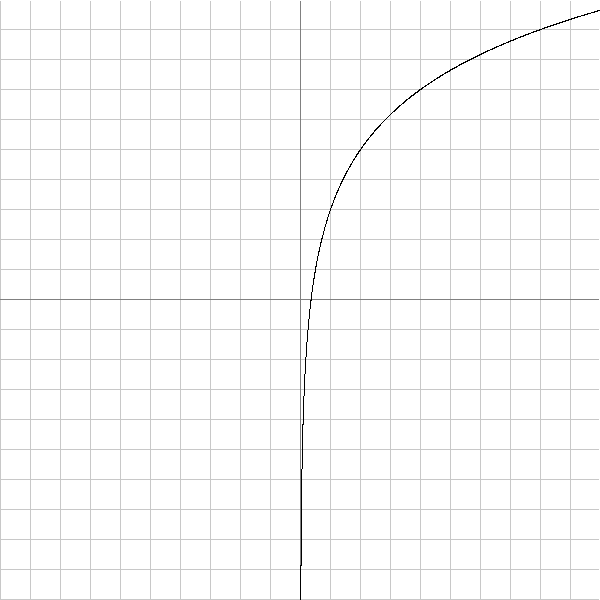
\includegraphics[scale=0.5]{graph.png}
\end{center}\section{Заключение}К данному моменту здравомыслящий читатель должен был осознать всю необходимость этой формулы. Особенно это открытие было важно для ремонта МФЦ в южной области Северодвинска. В противном случае, если смысл формулы понять не удалось, рекомендуется прочитать статью еще раз.\\\paragraph{Материалы и литература}\mbox{}\\
\begin{enumerate}\item\href{https://www.wolframalpha.com}{www.wolframalpha.com}\\
\item\href{https://github.com/JakMobius/MIPT-Tasks/tree/master/differentiator}{github.com/JakMobius/MIPT-Tasks/tree/master/differentiator}\\
\item\href{https://vk.com/ded32_ru}{vk.com/ded32\_ru}\\
\item\href{https://en.wikipedia.org/wiki/Special:Random}{bg.wikipedia.org/abduction\_date-palm\_climatic\_coompounda}\end{enumerate}\end{document}